\documentclass{homework}
\usepackage[utf8]{inputenc}
\usepackage{amsmath}
\usepackage{amssymb}
\usepackage{braket}
\usepackage{graphicx}

% CHANGE THE FOLLOW THREE LINES!
\newcommand{\hwname}{Vaansh Lakhwara}
\newcommand{\hwemail}{ID: 401147641}
\newcommand{\hwnum}{8}

% CHANGE THESE ONLY ONCE PER CLASS
\newcommand{\hwtype}{Assignment}
\newcommand{\hwclass}{COMP 335}

\begin{document}
\maketitle

\question
\textbf{(a)}\\
States q1,q2 take care of accepting b*, $\lambda$, while the path q3-q5 enforces $2i=k$, and path q3-q9 provides an alternative route by enforcing $i=j+1$.
\begin{center}
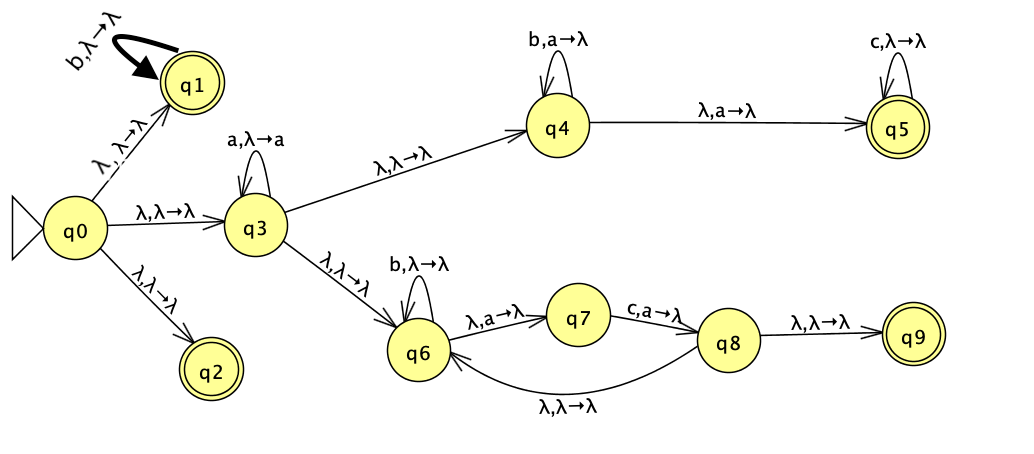
\includegraphics{a8_1.png}\\
\end{center}
\textbf{(b)}\\
if $n_a(w) = n_b(w)$, and for all prefixes of $w$ have $n_a(v) \geq n_b(v)$, then the strings accepted must have $b$ as the last letter, example: w = babaab, aaabbb, ababab, bbbaaaab, etc.
\begin{center}
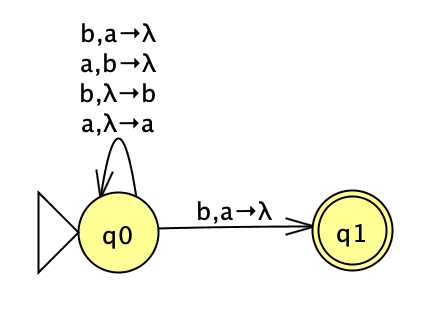
\includegraphics{a8_2.png}\\
\end{center}
\question
Converting the given CFG to an equivalent PDA, we get:
\begin{center}
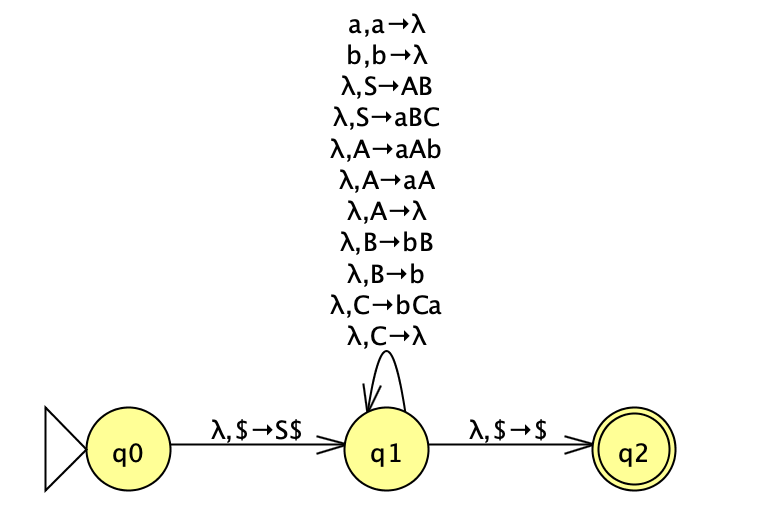
\includegraphics{a8_3.png}\\
\end{center}
\question
Accepts $\lambda$, or makes $0$ in multiples of 2/6s, so $1$ pops them appropriates in multiples of 3s.
\begin{center}
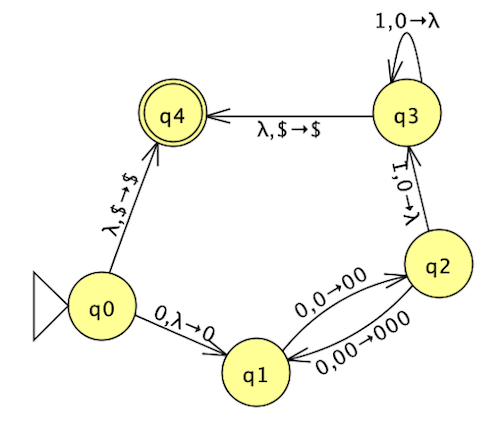
\includegraphics{a8_4.png}\\
\end{center}

\end{document}